% !TeX root = RJwrapper.tex
\title{gp3ml: Governance-First Predictive Modelling and Validation for Gazepoint Research in R}


\author{by Stefanos Balaskas}

\maketitle

\abstract{%
Predictive modelling with eye-tracking data is complicated by repeated participant--stimulus observations, heterogeneous recording quality, flexible preprocessing, and information leakage across resampling partitions. General machine-learning frameworks provide broad modelling functionality, but the scientific validity of a behavioural prediction workflow also depends on its declared outcome, grouping structure, generalization target, tuning boundaries, decision policy, and computational provenance. We introduce gp3ml, an R package for governance-first predictive modelling and validation with Gazepoint-derived and similarly structured research data. The package combines explicit task and feature-role declarations with participant-, stimulus-, trial-, and crossed-group resampling; fold-local preprocessing; nested tuning; retained assessment predictions; calibration and target-aware conformal summaries; threshold and abstention rules; shift and robustness audits; locked analysis plans; portable model artefacts; environment capture; research-object export; and explicit API contracts. An executable synthetic case study uses an observed recording-quality review status to compare row-level, participant-grouped, and participant--stimulus validation designs. The example generates every table and figure from deterministic code and reports design-specific performance rather than presuming that one split is universally correct. gp3ml is not an automatic model-selection system and does not infer hidden psychological, health, biometric, or sensitive attributes. Its contribution is an opinionated governance layer that links predictive modelling decisions to the units and claims a study is intended to support.
}

\section{Introduction}\label{introduction}

Eye-tracking experiments commonly produce multiple observations from each participant, repeated presentations of stimuli, and measurements nested within trials or recordings. These observations are not exchangeable rows in the ordinary sense: a classifier can exploit stable participant characteristics, recurring stimulus properties, or duplicated processing decisions when the same clusters occur in both training and assessment data. The corresponding issue is not limited to eye tracking. Crossed participant--item structures are foundational in behavioural research, and claims are normally intended to extend beyond the particular people, stimuli, or recordings observed in one sample \citep{Baayen2008, Barr2013, Yarkoni2022}.

A random row split can therefore answer a narrower question than its label suggests. It may estimate performance for additional rows drawn from already represented participants and stimuli, even when the scientific claim concerns new participants, new stimuli, or both. The resulting estimate is not intrinsically invalid; it is misaligned when it is interpreted as evidence for a different target. This distinction motivates the central design rule in \texttt{gp3ml}: the intended generalization unit is declared before folds are created, and fold construction preserves that declaration.

Leakage introduces a second problem. Information can cross the analysis--assessment boundary through outcome-derived features, post-outcome measurements, identifiers, globally estimated preprocessing, feature selection, tuning, or threshold optimization. Leakage has been defined as information about a prediction target that would not legitimately be available at prediction time \citep{Kaufman2012}. Its practical consequences extend beyond textbook mistakes: systematic reviews of machine-learning-based science have documented failures in which apparently strong performance depended on leakage or incomplete reporting \citep{Kapoor2023}.

Model selection requires a further boundary. Using the same resampling results both to choose a model and to report its expected performance can bias the estimate \citep{Varma2006, Cawley2010}. Nested resampling separates the inner selection problem from the outer performance-estimation problem. Yet nesting alone does not define which participants or stimuli may cross a partition, how preprocessing is estimated, what uncertainty is reported, or how a probability is converted into an action.

These concerns suggest that predictive validity is partly a governance problem. A defensible workflow must connect the outcome definition, feature provenance, resampling target, tuning rule, calibration method, threshold policy, robustness evidence, and computational environment. Performance metrics remain necessary, but they do not themselves establish that the analysis answered the intended question.

\texttt{gp3ml} \citep{gp3ml2026} implements this connection for Gazepoint-derived and similarly structured behavioural data. It provides modelling engines and evaluation utilities, but its distinctive purpose is to make design and reporting decisions explicit and auditable. The package does not autonomously identify a ``best'' model, relax prohibited-use boundaries, or treat predictive associations as evidence of latent mental states. This paper describes its architecture, positions it relative to existing R software, and provides a fully executable case study built around an explicitly observed recording-quality review status.

\section{Related software and methodological context}\label{related-software-and-methodological-context}

R already has mature modelling ecosystems. \texttt{caret} unified model training and resampling behind a common interface \citep{Kuhn2008}. \texttt{mlr3} provides an extensible object-oriented ecosystem for tasks, learners, resampling, tuning, and benchmarking \citep{Lang2019}. The \texttt{tidymodels} ecosystem integrates modelling components with tidy data principles \citep{KuhnSilge2022}, while \texttt{rsample} supplies general resampling infrastructure, including grouped and nested designs \citep{rsample2026}. These tools remain appropriate foundations for many analyses.

\texttt{gp3ml} is not positioned as a replacement for those systems. Its narrower contribution is to bind several decisions that researchers otherwise have to compose and document themselves: feature provenance, permitted outcomes, generalization targets, leakage audits, fold-local evaluation, human-recorded selection rationales, threshold provenance, abstention, dataset shift, environment comparison, portable artefacts, and API contracts. The package can use optional engines, but it deliberately restricts hidden automation and records when an optional runtime is unavailable. Other complementary tools address adjacent concerns: \texttt{DALEX} provides model-agnostic explainers \citep{Biecek2018}, while \texttt{targets} represents reproducible computational pipelines \citep{Landau2021}. \texttt{gp3ml} does not replace either function; it records governance evidence specific to the predictive research claim.

Eye-tracking packages address different parts of the workflow. \texttt{eyetrackingR}, for example, supports cleaning, aggregation, visualization, growth-curve analysis, onset-contingent analysis, and time-window methods \citep{DinkFerguson2015}. Such packages focus on deriving and analysing eye-tracking measures. \texttt{gp3ml} begins after an outcome and candidate predictors can be declared and asks how a predictive claim should be validated and documented.

Uncertainty and reporting also have established literatures. Conformal prediction constructs prediction sets or intervals under explicit exchangeability conditions \citep{Vovk2005, Shafer2008, Angelopoulos2023}. Calibration assesses whether predicted probabilities correspond to observed frequencies \citep{Guo2017}. Dataset-shift methods distinguish changes in covariates, prevalence, concepts, and performance rather than treating ``drift'' as one quantity \citep{QuioneroCandela2009, MorenoTorres2012}. Internal and external validation answer different questions and require explicit attention to the target setting \citep{Steyerberg2016}. Model cards encourage structured statements about purpose, evaluation, and limitations \citep{Mitchell2019}, while RO-Crate provides machine-readable packaging for research artefacts and their relationships \citep{SoilandReyes2022}. \texttt{gp3ml} integrates conservative forms of these ideas into one governed workflow without claiming that software alone resolves their assumptions.

\begin{table}
\centering
\caption{\label{tab:software-comparison-table}Scope-qualified comparison of selected R software. Entries describe primary documented scope rather than exhaustive capability.}
\centering
\resizebox{\ifdim\width>\linewidth\linewidth\else\width\fi}{!}{
\begin{tabular}[t]{llllll}
\toprule
Software & Primary\_scope & Grouped\_resampling & Leakage\_governance & Decision\_governance & Provenance\_portability\\
\midrule
gp3ml & Governed predictive research with clustered behavioural data & Native and target-labelled & Feature manifests and fold audits & Threshold provenance and abstention & Environment, artefacts, checksums, RO-Crate-oriented export\\
caret & General predictive modelling and resampling & Available through indices/control & Requires workflow composition & Requires external composition & Requires external composition\\
mlr3 & Extensible machine-learning tasks and benchmarking & Native & Requires workflow composition & Requires external composition & Requires external composition\\
tidymodels/rsample & Composable modelling and resampling workflows & Native & Requires workflow composition & Requires external composition & Requires external composition\\
DALEX & Model-agnostic explanation & Outside primary scope & Outside primary scope & Outside primary scope & Explanation objects\\
\addlinespace
targets & Reproducible computational pipelines & Requires external composition & Can orchestrate checks supplied by other tools & Outside primary scope & Native pipeline provenance and invalidation\\
eyetrackingR & Eye-tracking preparation and inferential analysis & Outside primary scope & Outside primary scope & Outside primary scope & Requires external composition\\
RO-Crate tooling & Packaging research objects and metadata & Outside primary scope & Outside primary scope & Outside primary scope & Native metadata packaging\\
\bottomrule
\end{tabular}}
\end{table}

\section{Design principles}\label{design-principles}

The package is organized around twelve principles (Table 2). The principles are constraints on interpretation as much as software features.

\begin{table}
\centering
\caption{\label{tab:design-principles-table}Design principles and representative package mechanisms.}
\centering
\resizebox{\ifdim\width>\linewidth\linewidth\else\width\fi}{!}{
\begin{tabular}[t]{lll}
\toprule
Principle & Operationalisation & Representative\_functions\\
\midrule
Declared purpose & Task and analysis-plan objects record the observed outcome and intended use. & declare\_gazepoint\_task(); declare\_gazepoint\_analysis\_plan()\\
Explicit roles & Outcome, predictors, identifiers and grouping columns are validated separately. & validate\_gazepoint\_ml\_roles()\\
Leakage-resistant validation & Feature manifests and fold audits identify unavailable, outcome-derived or overlapping information. & create\_gazepoint\_feature\_manifest(); audit\_gazepoint\_ml\_leakage()\\
Group-aware resampling & Participants, stimuli, trials or crossed blocks are held out according to the declared target. & create\_gazepoint\_group\_folds(); create\_gazepoint\_nested\_folds()\\
Target-aligned generalization & Every evaluation retains a machine-readable generalization target. & create\_gazepoint\_synthetic\_task(); validate\_gazepoint\_group\_folds()\\
\addlinespace
Fold-local preprocessing & Imputation, encoding, centring and scaling are estimated on analysis partitions. & fit\_gazepoint\_preprocessor(); evaluate\_gazepoint\_group\_folds()\\
Governed tuning & Candidate grids, selection metrics, directions and human rationales are explicit. & create\_gazepoint\_tuning\_grid(); select\_gazepoint\_model()\\
Uncertainty-aware evaluation & Fold distributions, calibration, bootstrap summaries and conformal caveats remain visible. & summarize\_gazepoint\_resample\_performance(); fit\_gazepoint\_conformal()\\
Explicit decisions & Threshold source, costs and abstention intervals are represented as validated objects. & evaluate\_gazepoint\_thresholds(); create\_gazepoint\_decision\_rule()\\
Reproducible evidence & Plans, environments, checksums, reports and release evidence can be audited. & lock\_gazepoint\_analysis\_plan(); capture\_gazepoint\_environment()\\
\addlinespace
Portable artefacts & Model and preprocessing components can be validated and restored as governed artefacts. & create\_gazepoint\_model\_artifact(); validate\_gazepoint\_model\_artifact()\\
Bounded scope and API contracts & Prohibited interpretations and stable/experimental interfaces are explicit. & gp3ml\_prohibited\_uses(); gp3ml\_api\_contracts()\\
\bottomrule
\end{tabular}}
\end{table}

\section{Package architecture}\label{package-architecture}

The architecture is layered rather than tied to one learner (Figure 1). Task declarations and feature manifests precede resampling. Preprocessing and model fitting are evaluated inside materialized partitions. Uncertainty, shift and decision rules consume retained predictions. Artefacts and API contracts preserve the resulting evidence.

\begin{verbatim}
plot_architecture()
\end{verbatim}

\begin{figure}

{\centering 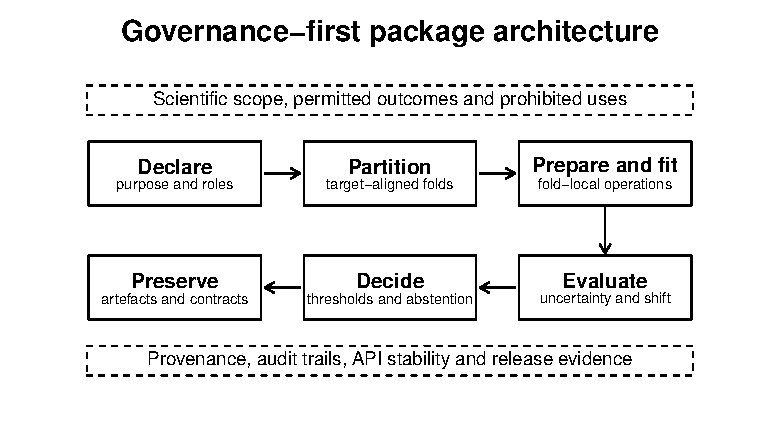
\includegraphics[width=0.88\linewidth,alt={Six workflow boxes connected by arrows, from purpose and roles through grouped resampling and modelling to artefacts and API contracts.}]{gp3ml-paper_files/figure-latex/architecture-figure-1}

}

\caption{Conceptual architecture of gp3ml. Governance begins before model fitting and continues through release evidence.}\label{fig:architecture-figure}
\end{figure}

At render time, the manuscript audits the installed source rather than relying on manually copied counts. The current source identifies version 0.3.0, 71 stable exports, 56 experimental exports, and 38 stable public classes. The API audit status is pass with 0 recorded differences. The repository contains 20 source vignettes and 154 Rd topics.

\begin{table}
\centering
\caption{\label{tab:package-facts-table}Dynamically audited package facts and fixed release evidence.}
\centering
\resizebox{\ifdim\width>\linewidth\linewidth\else\width\fi}{!}{
\begin{tabular}[t]{ll}
\toprule
Item & Evidence\\
\midrule
Package version & 0.3.0\\
Namespace exports & 127\\
Stable exports & 71\\
Experimental exports & 56\\
Stable public classes & 38\\
\addlinespace
API audit & pass with 0 differences\\
Source vignettes & 20\\
Rd topics & 154\\
GitHub tag & v0.3.0 at 0e23684f32a44417827aa0e7fee9fefc9e6c35d3\\
Validated archive SHA-256 & 04c5fdb017c63ecbf6f5e85c29fff6492880201a2f2aa5c3c1d3fe998e60bae6\\
\addlinespace
CRAN status at drafting & 0.3.0 is a GitHub source release; CRAN submission is pending\\
\bottomrule
\end{tabular}}
\end{table}

The modelling engines are not assumed to be interchangeable. Their runtime status is queried when the paper is rendered, and optional dependencies are reported rather than treated as silently available.

\begin{table}
\centering
\caption{\label{tab:engine-capability-table}Runtime-audited modelling-engine capabilities in the rendering environment.}
\centering
\resizebox{\ifdim\width>\linewidth\linewidth\else\width\fi}{!}{
\begin{tabular}[t]{llll}
\toprule
engine & package & status & notes\\
\midrule
glm & NA & available & Base-R binomial GLM.\\
lm & NA & available & Base-R linear model.\\
ranger & ranger & available & Optional package; governed wrapper.\\
xgboost & xgboost & available & Optional package; governed wrapper.\\
nnet & nnet & available & Recommended R package; governed wrapper.\\
\addlinespace
keras3 & keras3 & unavailable & Optional package plus configured backend; deep learning remains explicit.\\
custom & NA & available & Externally supplied engine requires safety declarations.\\
\bottomrule
\end{tabular}}
\end{table}

At render time, 11 of 13 declared optional dependencies were available. The complete runtime matrix is supplied in \texttt{paper/supplement/optional-dependencies.csv}.

\section{Synthetic research case study}\label{synthetic-research-case-study}

\subsection{Data-generating design}\label{data-generating-design}

The case study uses \texttt{simulate\_gazepoint\_governed\_data()}, which generates deterministic, non-sensitive participant--stimulus trials with explicit outcomes. We use the predefined \texttt{quality\_status} factor as the outcome. It records whether a synthetic trial has been assigned a \emph{pass} or \emph{review} recording-quality status; it is not a psychological construct. The predictors are \texttt{tracking\_ratio}, \texttt{blink\_rate}, and \texttt{gaze\_dispersion}. Five per cent of \texttt{gaze\_dispersion} values are then set to missing using a fixed seed. This perturbation tests whether imputation remains inside analysis folds.

\begin{table}
\centering
\caption{\label{tab:synthetic-data-structure}Synthetic case-study structure.}
\centering
\resizebox{\ifdim\width>\linewidth\linewidth\else\width\fi}{!}{
\begin{tabular}[t]{ll}
\toprule
Component & Value\\
\midrule
Rows & 480\\
Participants & 30\\
Stimuli & 8\\
Trials per participant–stimulus cell & 2\\
Outcome & quality\_status\\
\addlinespace
Positive class & review\\
Predictors & tracking\_ratio, blink\_rate, gaze\_dispersion\\
Controlled missingness & 24 gaze\_dispersion values (5\%)\\
\bottomrule
\end{tabular}}
\end{table}

The feature manifest records that the predictors are available during exposure, are not outcome-derived, and require fold-local preprocessing. The task declares prediction for new participants. A separate task is constructed for simultaneous participant and stimulus generalization; the outcome and predictors do not change, but the held-out units do.

\subsection{Locked analysis plan}\label{locked-analysis-plan}

The plan fixes the outcome, predictors, target, preprocessing, candidate model, primary metric, uncertainty method, and prohibited interpretations before the model results are inspected.

\begin{table}
\centering
\caption{\label{tab:analysis-plan-code}Locked analysis-plan summary.}
\centering
\resizebox{\ifdim\width>\linewidth\linewidth\else\width\fi}{!}{
\begin{tabular}[t]{ll}
\toprule
Element & Evidence\\
\midrule
Validation & pass\\
Outcome & quality\_status\\
Generalization target & new\_participants\\
Predictors & tracking\_ratio, blink\_rate, gaze\_dispersion\\
Preprocessing & Median imputation, centring and scaling within analysis folds\\
\addlinespace
Candidate model & glm\\
Primary metric & balanced\_accuracy\\
Locked plan & gp3ml-plan-cca872151af2\\
\bottomrule
\end{tabular}}
\end{table}

A valid plan does not prove that its scientific choices are correct. It creates an immutable reference against which changes can be reported. This operationalizes the distinction between decisions declared before results are inspected and changes made after observation, without claiming that a software lock is equivalent to a registered preregistration \citep{Nosek2018}. In this execution, the final configuration is compared with the locked plan rather than silently substituting a different metric or target.

\subsection{Validation designs}\label{validation-designs}

Three designs are compared. The row-level comparator deliberately allows cluster overlap and is implemented as manuscript-specific code because \texttt{gp3ml} does not offer an unlabeled unsafe split as a governed target. The second design assigns complete participants to assessment folds. The third creates crossed participant--stimulus assessment blocks and retains incompatible cross-block rows as excluded rather than silently moving them.

\begin{verbatim}
plot_resampling_schemes(analysis_data, group_folds, cross_folds)
\end{verbatim}

\begin{figure}

{\centering 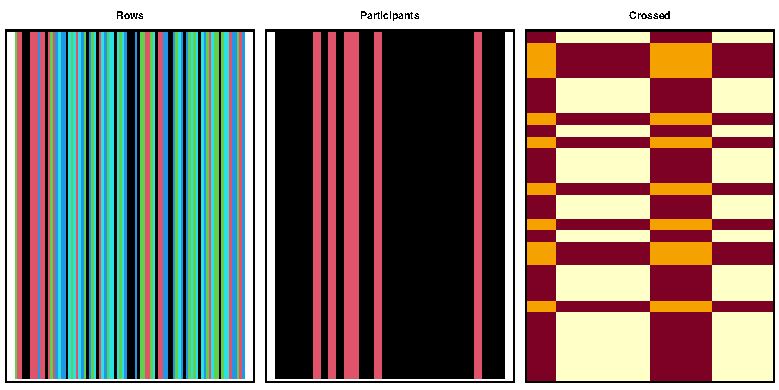
\includegraphics[width=0.86\linewidth,alt={Three panels showing row-level colour blocks, participants assigned wholly to one partition, and participant-by-stimulus assessment blocks with excluded cross-block cells.}]{gp3ml-paper_files/figure-latex/resampling-design-figure-1}

}

\caption{Three validation designs applied to the same synthetic data. The first is an intentionally unsafe comparator; the latter two are materialized by gp3ml.}\label{fig:resampling-design-figure}
\end{figure}

\begin{table}
\centering
\caption{\label{tab:validation-design-table}Validation designs and their interpretation.}
\centering
\resizebox{\ifdim\width>\linewidth\linewidth\else\width\fi}{!}{
\begin{tabular}[t]{lllllll}
\toprule
Design & Intended\_estimand & Same\_participant\_across\_sides & Same\_stimulus\_across\_sides & Fold\_local\_preprocessing & Excluded\_cross\_block\_rows & Leakage\_audit\\
\midrule
Naive row-level & Additional rows from represented clusters & Possible & Possible & Yes, in comparator code & None & Not governed\\
Participant grouped & New participants with represented stimulus set & Prevented & Possible & Yes, through gp3ml & None & pass\\
Participant–stimulus blocks & New participant–stimulus blocks & Prevented for assessment block & Prevented for assessment block & Yes, through gp3ml & 1920 & pass\\
\bottomrule
\end{tabular}}
\end{table}

\section{End-to-end governed workflow}\label{end-to-end-governed-workflow}

The participant-grouped workflow materializes folds, audits cluster separation, estimates median imputation, centring and scaling inside each analysis partition, fits a logistic regression, and retains only assessment predictions. The model is deliberately simple: the paper evaluates workflow semantics rather than claiming algorithmic superiority.

\begin{table}
\centering
\caption{\label{tab:grouped-workflow-code}Participant-grouped workflow audit.}
\centering
\resizebox{\ifdim\width>\linewidth\linewidth\else\width\fi}{!}{
\begin{tabular}[t]{ll}
\toprule
Component & Evidence\\
\midrule
Target & new\_participants\\
Materialized folds & 10\\
Fold audit & pass\\
Evaluation validation & pass\\
Assessment predictions & 960\\
\addlinespace
Failed folds & 0\\
\bottomrule
\end{tabular}}
\end{table}

Nested tuning is available through \texttt{create\_gazepoint\_nested\_folds()} and \texttt{evaluate\_gazepoint\_nested\_resampling()}. It is not repeated in the main case study because only one learner is needed to isolate the effect of the validation target. The package's nested workflow records the inner metric, direction, success threshold, and human rationale for each outer fold; it should be used when candidate models or hyperparameters are selected.

\section{Results}\label{results}

\subsection{Validation-design dependence}\label{validation-design-dependence}

The metrics below are generated from the same data and predictor set. They should not be interpreted as a benchmark of logistic regression. Their purpose is to show that ``model performance'' is conditional on which units were permitted to recur across analysis and assessment data.

\begin{table}
\centering
\caption{\label{tab:performance-summary-table}Fold-distribution summaries by validation design.}
\centering
\resizebox{\ifdim\width>\linewidth\linewidth\else\width\fi}{!}{
\begin{tabular}[t]{lllrrrrr}
\toprule
  & design & metric & n\_folds & mean & sd & lower & upper\\
\midrule
4 & Naive row-level & balanced\_accuracy & 10 & 0.500 & 0.000 & 0.500 & 0.500\\
5 & Participant-stimulus blocks & balanced\_accuracy & 9 & 0.500 & 0.000 & 0.500 & 0.500\\
6 & Participant grouped & balanced\_accuracy & 10 & 0.500 & 0.000 & 0.500 & 0.500\\
29 & Naive row-level & roc\_auc & 10 & 0.603 & 0.075 & 0.493 & 0.698\\
30 & Participant-stimulus blocks & roc\_auc & 9 & 0.618 & 0.062 & 0.507 & 0.688\\
\addlinespace
31 & Participant grouped & roc\_auc & 10 & 0.593 & 0.065 & 0.487 & 0.689\\
7 & Naive row-level & brier & 10 & 0.126 & 0.022 & 0.099 & 0.164\\
8 & Participant-stimulus blocks & brier & 9 & 0.123 & 0.042 & 0.058 & 0.180\\
9 & Participant grouped & brier & 10 & 0.128 & 0.028 & 0.082 & 0.163\\
16 & Naive row-level & log\_loss & 10 & 0.418 & 0.058 & 0.347 & 0.526\\
\addlinespace
17 & Participant-stimulus blocks & log\_loss & 9 & 0.415 & 0.109 & 0.246 & 0.546\\
18 & Participant grouped & log\_loss & 10 & 0.423 & 0.069 & 0.315 & 0.517\\
\bottomrule
\end{tabular}}
\end{table}

\begin{verbatim}
plot_validation_profile(all_metrics, performance_summary)
\end{verbatim}

\begin{figure}

{\centering 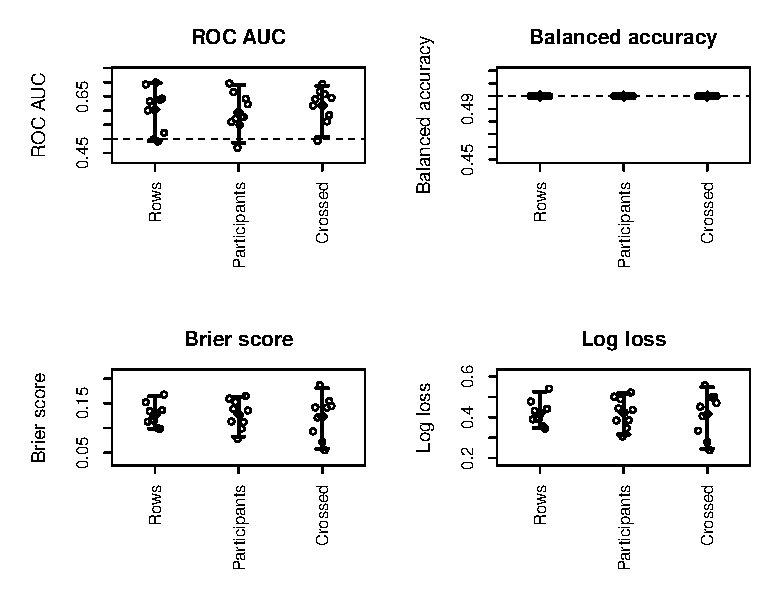
\includegraphics[width=0.88\linewidth,alt={Four panels compare ROC AUC, balanced accuracy, Brier score and log loss across row-level, participant-grouped and crossed participant-stimulus validation.}]{gp3ml-paper_files/figure-latex/performance-comparison-figure-1}

}

\caption{Multi-metric validation profile for the three declared generalization designs. Open points are fold estimates; filled diamonds are means and vertical segments are empirical 95\% fold-distribution intervals. Similar numerical values do not make the three estimands interchangeable.}\label{fig:performance-comparison-figure}
\end{figure}

The executable result should be read design by design. A higher row-level value would be evidence that repeated cluster information makes the row-level problem easier, not proof that the grouped estimate is pessimistic. Conversely, similar values would show that the selected predictors do not rely strongly on cluster recurrence in this synthetic realization. The code does not force either conclusion.

\subsection{Calibration and conformal sets}\label{calibration-and-conformal-sets}

Calibration is assessed from retained participant-grouped assessment predictions from the first repeated-CV pass, so each source row appears once in this diagnostic. The reliability plot is descriptive; repeated trials from the same participant mean that ordinary row-bootstrap intervals are not treated as participant-level uncertainty.

\begin{table}
\centering
\caption{\label{tab:calibration-summary-table}Calibration summary for participant-grouped assessment predictions.}
\centering
\resizebox{\ifdim\width>\linewidth\linewidth\else\width\fi}{!}{
\begin{tabular}[t]{rrrrr}
\toprule
intercept & slope & brier & log\_loss & ece\\
\midrule
-0.755 & 0.547 & 0.128 & 0.425 & 0.021\\
\bottomrule
\end{tabular}}
\end{table}

\begin{verbatim}
plot_calibration_conformal(calibration, conformal_coverage, conformal_set_size)
\end{verbatim}

\begin{figure}

{\centering 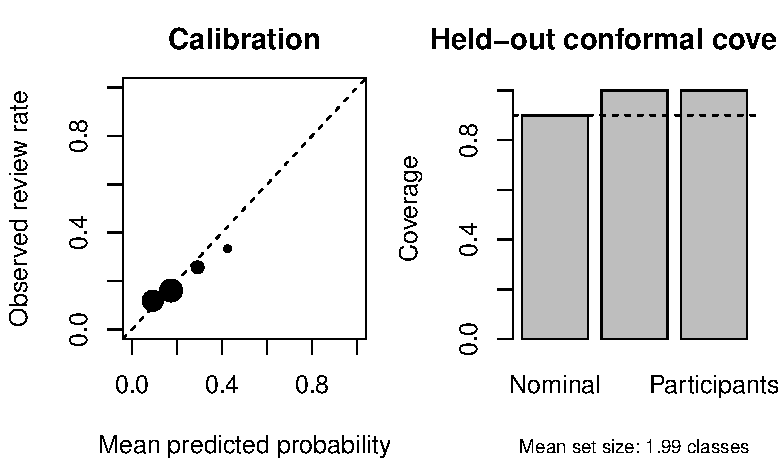
\includegraphics[width=0.88\linewidth,alt={Two panels show a calibration reliability diagram and held-out conformal coverage for rows and participants.}]{gp3ml-paper_files/figure-latex/calibration-figure-1}

}

\caption{Calibration and participant-disjoint conformal uncertainty. The left panel compares predicted and observed review rates; the right panel compares nominal, row-level and participant-level held-out coverage, with mean prediction-set size reported beneath the panel.}\label{fig:calibration-figure}
\end{figure}

The conformal example first divides the retained assessment predictions into participant-disjoint policy-development and policy-audit partitions. Conformity scores are estimated only from the development participants and aggregated to participants before the quantile is estimated; prediction sets are then evaluated on the held-out participants. The implementation records this calibration unit and a caveat: coverage claims still require exchangeability assumptions appropriate to the declared target. The observed held-out row coverage is 1, the all-rows-covered participant proportion is 1, and the mean prediction-set size is 1.988 classes at nominal coverage 0.9.

\begin{table}
\centering
\caption{\label{tab:conformal-summary-compact}Participant-disjoint conformal summary.}
\centering
\resizebox{\ifdim\width>\linewidth\linewidth\else\width\fi}{!}{
\begin{tabular}[t]{rrrrrrl}
\toprule
development\_participants & audit\_participants & nominal\_coverage & held\_out\_row\_coverage & held\_out\_participant\_coverage & mean\_set\_size & status\\
\midrule
15 & 15 & 0.9 & 1 & 1 & 1.988 & pass\\
\bottomrule
\end{tabular}}
\end{table}

\subsection{Threshold and abstention governance}\label{threshold-and-abstention-governance}

A probability estimate is not a decision rule. Candidate thresholds are explicit, the optimization metric and direction are recorded, and the selected threshold carries a declared provenance. In the executable demonstration, the threshold and the abstention interval are developed on one participant subset and audited on disjoint held-out participants. The interval between 0.15 and 0.25 is centred on the deterministic selected threshold and is used only to demonstrate auditable selective prediction; it is not an operational recommendation.

\begin{table}
\centering
\caption{\label{tab:decision-rule-code}Governed decision-policy summary.}
\centering
\resizebox{\ifdim\width>\linewidth\linewidth\else\width\fi}{!}{
\begin{tabular}[t]{ll}
\toprule
Element & Evidence\\
\midrule
Rule validation & pass\\
Threshold & 0.2\\
Threshold origin & training\\
Generalization target & new\_participants\\
Held-out coverage & 0.621\\
\addlinespace
Held-out abstention & 0.379\\
Covered error & 0.221\\
\bottomrule
\end{tabular}}
\end{table}

\begin{verbatim}
plot_threshold_and_abstention(threshold_evaluation, decision_rule, policy_audit_predictions, quality_task$positive, abstention_audit)
\end{verbatim}

\begin{figure}

{\centering 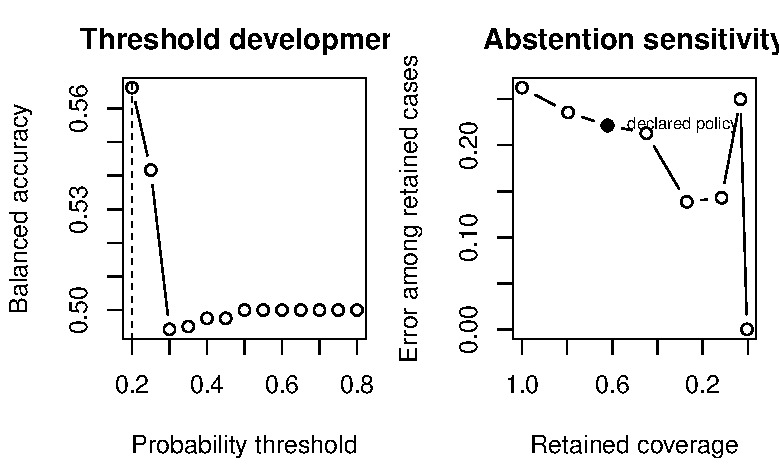
\includegraphics[width=0.88\linewidth,alt={Two panels show balanced accuracy across thresholds and the trade-off between retained coverage and error after abstention.}]{gp3ml-paper_files/figure-latex/threshold-abstention-figure-1}

}

\caption{Threshold development and abstention sensitivity on participant-disjoint data. The left panel marks the selected threshold; the right panel shows the retained-coverage versus covered-error frontier across symmetric abstention bands and highlights the declared policy.}\label{fig:threshold-abstention-figure}
\end{figure}

\subsection{Dataset shift and robustness}\label{dataset-shift-and-robustness}

A second synthetic dataset is perturbed transparently: \texttt{tracking\_ratio} is shifted downward, \texttt{gaze\_dispersion} is scaled, and its missingness increases. \texttt{audit\_gazepoint\_dataset\_shift()} reports numeric standardized differences or categorical total variation together with support overlap and outside-range rates. Missingness is audited separately so that one score does not conflate distinct phenomena.

\begin{table}
\centering
\caption{\label{tab:shift-table}Concise predictor-distribution shift findings.}
\centering
\resizebox{\ifdim\width>\linewidth\linewidth\else\width\fi}{!}{
\begin{tabular}[t]{lrrrrrl}
\toprule
predictor & mean\_development & mean\_external & standardized\_difference & support\_overlap & outside\_training\_range & status\\
\midrule
tracking\_ratio & 0.914 & 0.838 & -1.974 & 0.830 & 0.170 & fail\\
blink\_rate & 5.869 & 6.165 & 0.221 & 0.997 & 0.003 & review\\
gaze\_dispersion & 0.786 & 0.982 & 1.503 & 0.785 & 0.215 & fail\\
\bottomrule
\end{tabular}}
\end{table}

\begin{verbatim}
plot_shift(shift_audit)
\end{verbatim}

\begin{figure}

{\centering 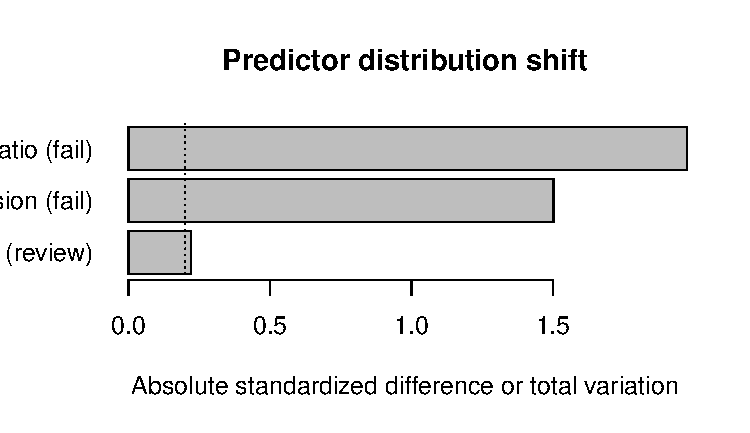
\includegraphics[width=0.86\linewidth,alt={Horizontal bars showing shift magnitude for tracking ratio, blink rate, and gaze dispersion.}]{gp3ml-paper_files/figure-latex/shift-figure-1}

}

\caption{Predictor distribution shift between development and perturbed synthetic external data.}\label{fig:shift-figure}
\end{figure}

\begin{table}
\centering
\caption{\label{tab:robustness-code}Seed and threshold sensitivity audit.}
\centering
\resizebox{\ifdim\width>\linewidth\linewidth\else\width\fi}{!}{
\begin{tabular}[t]{llrl}
\toprule
dimension & metric & indicator & status\\
\midrule
seed & balanced\_accuracy & 0.009 & pass\\
threshold & balanced\_accuracy & 0.000 & fail\\
\bottomrule
\end{tabular}}
\end{table}

The seed and threshold diagnostics are not substitutes for external validation. They expose whether a reported result is highly contingent on fold allocation or threshold choice within the evaluated design.

\subsection{Plan, artefact and environment validation}\label{plan-artefact-and-environment-validation}

The actual configuration matches the locked plan with status pass. The model artefact validation status is pass, the environment self-comparison status is pass, and the API stability audit status is pass.

\begin{table}
\centering
\caption{\label{tab:governance-validation-table}Governance and reproducibility evidence generated by the case study.}
\centering
\resizebox{\ifdim\width>\linewidth\linewidth\else\width\fi}{!}{
\begin{tabular}[t]{lll}
\toprule
Evidence & Status & Detail\\
\midrule
Locked plan & locked & gp3ml-plan-cca872151af2\\
Plan-deviation audit & pass & 0 declared deviations\\
Decision rule & pass & threshold 0.2 from training\\
Model artefact & pass & Unbundled representative fold model with governed metadata\\
Environment comparison & pass & Captured environment compared with itself as a deterministic validation check\\
\addlinespace
API stability & pass & 0 differences\\
\bottomrule
\end{tabular}}
\end{table}

\section{Software quality and validation}\label{software-quality-and-validation}

The 0.3.0 release was checked from its exact source archive with all declared \texttt{Suggests} packages available. The release workflow recorded zero errors, zero warnings, and zero notes; rebuilt all source vignettes; generated PDF and HTML manuals; and found no CRAN reverse dependencies at the time of the audit. The archive SHA-256 is reported in the package-facts table. These are release facts, not claims that every scientific use of the package is valid.

The manuscript adds a second validation layer. \texttt{paper/R/render-paper.R} installs the repository into a temporary library before rendering, so the user's installed package is not overwritten. \texttt{paper/R/validate-paper.R} distinguishes passed checks, failed checks, unavailable optional diagnostics, and checks not evaluated. It runs the manuscript render, package tests, \texttt{pkgdown::check\_pkgdown()}, API audit, scope-language audit, and a Git working-tree boundary check. This emphasis follows broader calls for executable artefacts, transparent checklists, and reproducibility reporting in machine-learning research \citep{Pineau2021}. The R Journal recommends the \texttt{rjtools} template, reproducible code and data, alt text for figures, and pre-submission checks; this workspace follows that structure.

\section{Discussion}\label{discussion}

\texttt{gp3ml} treats governance as part of predictive validity. This position does not imply that every analysis requires the same split, model, metric, or decision rule. It implies that these choices define the claim being made and should therefore be explicit, machine-readable, and reviewable.

The generalization target is the organizing decision. Holding out participants estimates a different problem from holding out stimuli or crossed participant--stimulus blocks. A row-level split can be appropriate for additional rows from known clusters, but it should not be described as evidence for new participants without further justification. Materialized folds make this distinction inspectable: researchers can see analysis, assessment, and excluded rows rather than relying on an opaque resampling label.

The same principle applies to preprocessing and tuning. Median imputation may appear innocuous, yet a median estimated globally includes information from assessment rows. \texttt{gp3ml} passes preprocessing arguments into each fold's analysis partition. Candidate tuning grids and nested folds extend the separation to model selection. Human review remains necessary because a numerically optimal candidate may be inappropriate for the scientific purpose, effective sample size, interpretability requirement, or deployment context.

Decision governance prevents another common collapse. Calibration, discrimination, threshold selection, and abstention answer different questions. A well-ranked model can have poorly calibrated probabilities; a calibrated probability still requires costs or scientific priorities before it becomes a decision. The package therefore records the threshold's origin, training partition, metric, direction, costs, target, and justification. Abstention is represented as a measurable loss of coverage rather than hidden as missing output.

The package complements broader R frameworks. Researchers needing extensive learner catalogues, sophisticated search spaces, or distributed benchmarking may use \texttt{mlr3}, \texttt{tidymodels}, or other infrastructure and then adapt their outputs to a governed reporting layer. Conversely, the package's functions can support transparent studies using simple generalized linear models. The contribution is the integrity of the workflow, not model complexity.

Although the package was developed around Gazepoint-derived research data, its grouping and governance abstractions are not tied to a file format or device. Any tabular behavioural dataset with declared outcomes, predictors, participants, stimuli, trials, or other clusters can use the same logic. Device-specific preprocessing should occur upstream and be documented in the feature manifest and handoff objects.

\section{Limitations}\label{limitations}

Software governance cannot repair a weak research design, an invalid outcome, inadequate measurement, or a sample that does not represent the intended population. A passing leakage audit means that the encoded checks passed; it does not prove that every causal or temporal dependency has been identified.

Grouped validation can reveal that the effective sample size is much smaller than the row count. With few participants or stimuli, fold estimates can be unstable or some assessment folds can lack a class. \texttt{gp3ml} retains warnings and failed folds rather than silently discarding them, but the researcher must respond through redesign, simpler claims, or additional data.

The case study is synthetic. It demonstrates execution and interpretation but does not establish performance across real eye-tracking studies, devices, tasks, populations, or recording conditions. Broader empirical benchmarking with independent datasets is future work.

Conformal summaries depend on exchangeability assumptions and on how calibration units are defined. Group aggregation is conservative but does not provide distribution-free guarantees under arbitrary dependence. Dataset-shift audits describe measured differences; they do not identify a causal source of drift or guarantee performance degradation.

Optional modelling engines differ in installation requirements and supported tasks. The package reports capability status rather than treating an unavailable runtime as a core failure. The framework does not automate scientific judgment, does not perform unrestricted automated model selection, and does not infer emotion, stress, cognition, diagnosis, identity, protected attributes, or other hidden sensitive states.

\section{Availability and reproducibility}\label{availability-and-reproducibility}

\texttt{gp3ml} is released under the licence reported dynamically from \texttt{DESCRIPTION} (MIT + file LICENSE). Version 0.3.0 is archived as GitHub tag \texttt{v0.3.0} and is documented at \url{https://stefanosbalaskas.github.io/gp3ml/}. The repository is \url{https://github.com/stefanosbalaskas/gp3ml}. The Zenodo concept DOI is \url{https://doi.org/10.5281/zenodo.21487272}; a version-specific DOI should replace the placeholder in the final accepted manuscript once assigned. At the date of this draft, 0.3.0 is a GitHub source release and is not described as a CRAN release.

All examples use deterministic synthetic data generated during rendering with R \citep{R2026}. The source manuscript, helper scripts, evidence table, generated tables, validation script, and motivation letter are contained under \texttt{paper/}. The R Journal render script installs the current repository in a temporary library, writes the PDF and generated TeX to \texttt{paper/}, and writes the self-contained web article to \texttt{paper/output/}; \texttt{paper/R/render-preview.R} creates an HTML preview from the same executable source. No private participant data are included.

\appendix

The full executed function inventory, locked-plan printout, workflow-object printouts, and rendering session information are regenerated into \texttt{paper/supplement/} by the hidden chunk below; they are omitted from the main article to preserve the 20-page limit.

\bibliography{references.bib}

\address{%
Stefanos Balaskas\\
eGovernment \& eCommerce Lab (Innovation \& Entrepreneurship), Department of Business Administration\\%
University of Patras, 26504 Patras, Greece\\
%
\url{https://sites.google.com/view/stefbalaskas/}\\%
\textit{ORCID: \href{https://orcid.org/0000-0003-2444-9796}{0000-0003-2444-9796}}\\%
\href{mailto:s.balaskas@ac.upatras.gr}{\nolinkurl{s.balaskas@ac.upatras.gr}}%
}
